
\chapter{Experiments}
\label{chp:exp}

\hspace{0.1in}
\begin{section}{Offline Experiments}\label{sec:offline}
  \begin{subsection}{Datasets}


\begin{itemize}

\item \textbf{Yixun}: A dataset from Yixun\footnote{http://www.yixun.com}, a large online retailer for electronic products, that has been sampled from log data from two weeks(20130801 to 20130814). For click and purchase behaviors, we created a subset for which there are at least 10 interactions per user and item. 
\item \textbf{Tmall}: A similar but smaller anonymized dataset from a shopping portal\footnote{http://www.tmall.com} containing user interactions of different types(click and purchase). For each of the actions, a time stamp is available. It is a relatively long-term data, actions are recorded from 20140103 to 20140704. 
\end{itemize}

\begin{table}
\begin{center}
  \begin{tabular}{c c c}
    \hline
    Datasets & Yixun & Tmall\\
    \hline
    users(click) & 16,240 & 884\\
    %\hline
    items(click) & 1,932 & 9,531\\
    %\hline
    sparsity(click) & 0.006 & 0.021\\
    %\hline
    \hline
    users(purchase) & 2,520& 840\\
    %\hline
    item(purchase) & 1,791& 4,312\\
    %\hline
    sparsity(purchase) & 0.0003 & 0.001\\
\hline
  \end{tabular}
\end{center}
\caption{Dataset characteristics.}
\label{dataset}


\end{table}
\end{subsection}



\begin{subsection}{Metrics}
We use $prec@5$ and $prec@10$ as our evaluation metrics. Precision is the fraction of clicked items that are shown to the user. $$Precision = \frac{\|clicked items\| \cap \|shown items\|}{\|shown items\|}$$Precision takes all retrieved documents into account, but it can also be evaluated at a given cut-off rank, considering only the topmost results returned by the system. This measure is called \textbf{precision at n} or \textbf{$prec@n$}. $prec@n$ is widely used in information retrieval for evaluating the ranked documents over a set of queries. We use it to assess the overall performance based on precisions at different recall levels on a test set. It computes the mean of precision over all users in the test set. 

In the Yixun dataset, data from the first week is used as training data while we perform testing on data from the second week. For Tmall dataset, we select the last five purchased items from each user as their test data while training on their previous data.

Our main goal is to optimize for the conversion rate (future purchase matrix), so the test is mainly done in the purchase matrix. However, since TRIMF can also optimize for the source domain (click matrix), some tests in the click matrix are also conducted.

  
\end{subsection}

\begin{subsection}{Baseline Methods}  

We divide baseline methods into non-transfer methods and transfer methods. All baseline methods are shown in Table \ref{baseline}.
\begin{table}

\begin{center}
  \begin{tabular}{|c|c|}
    \hline
    non-transfer methods & transfer methods\\
    \hline
    Most Popular, SVD, NMF, PMF, BPRMF, WRMF&CMF, TCF\\
\hline
  \end{tabular}
\end{center}
\caption{Baseline methods.}
\label{baseline}


\end{table}
\subsubsection{non-transfer methods}
\par{
  For all non-transfer methods, we use three combinations of matrices as our training matrix:{deal, click, deal+click}, and report their \textbf{best} performance. We choose parameters by cross validation.
  \begin{itemize}
    \item Most Popular: selects top-n items globally, and provides the same recommendation results for every user.
    \item Singular Value Decomposition(SVD) ~\cite{paterek07}:  is a typical method used in recommender system, here PureSVD from Matlab is used.
      \begin{itemize}
      \item rank = \{5,10,20,30,40,50\}
      \end{itemize}
    \item Non-negative Matrix Factorization(NMF)  ~\cite{/computer/yehuda09matrix}: is also a typical method used in recommender system, here NMF from Matlab is used.
      \begin{itemize}
      \item rank = \{10,20,40,60,100\}
      \end{itemize}
    \item Probabilistic Matrix Factorization(PMF) ~\cite{/nips/SalMnih08}: is a recently proposed method for missing value prediction. Previous work showed that this method worked well on the large, sparse and imbalanced dataset.
      \begin{itemize}
      \item rank = \{10,20,30,40,50\}
      \end{itemize}
    \item BPRMF ~\cite{Rendle:2009:BBP:1795114.1795167}: BPR is a generic optimization criterion for personalized ranking. It is a maximum posterior estimator derived from a Bayesian analysis of the problem. Unlike traditional methods whose objective function is point-wise, BPR is a pair-wise object function. BPRMF implements BPR using matrix factorization.
      \begin{itemize}
      \item We initialized BPR with the most popular results.
      \item We set $iteration = \#n * 100$, ($\#n$ in the number of observations)
      \end{itemize}
    \item WRMF ~\cite{4781145}: One-class collaborative filtering(WRMF) is a weighted low rank approximation method optimized for an implicit dataset. 
      \begin{itemize}
      \item rank = \{5,10,15,20,25\}
    \end{itemize}
\end{itemize}
\subsubsection{transfer methods}
\begin{itemize}
    \item Collective Matrix Factorization(CMF) ~\cite{/kdd/SinghG08}: is proposed for jointly factorizing two matrices. Adopted as a transfer
learning technique in several recent works, CMF has been proven to be an effective cross-domain recommendation approach. For each training and testing pairs, we make two matrices of the same dimensions(in order to share a latent factor) by padding zero rows \& columns.
      \begin{itemize}
      \item Shared latent space dimension = \{5,10,15,20,25\}
      \end{itemize}
    \item TCF ~\cite{/ijcai/PanLXY11}: is a transfer learning method used to predict missing ratings via heterogeneous feedback. It is originally designed for rating prediction, so we set the deal matrix with randomly sampled zeros as the rating matrix, and click matrix as the implicit feedback matrix. Zero rows and columns are also padded to make the two matrices of the same dimensions.
\end{itemize}
\subsubsection{our methods}
\begin{itemize}
\item TRIMF
  \begin{itemize}
  \item We set latent factor = 30, iteration = 200.
  \end{itemize}
  \item CBMF
  \begin{itemize}
  \item We set latent factor = 15, iteration = 200, and we run Minhash for five times and concatenate them as our cluster id.
  \end{itemize}
    \end{itemize}
  
}
\end{subsection}
\end{section}
\subsection{Results}
  \begin{subsubsection}{Yixun}
\par{The user overlap of the deal and click matrix are small, so we perform two tests, one on deal matrix $X_d$ and one on click matrix $X_c$.}
\par{Results are shown in Tables \ref{shortdeal} and \ref{shortclick}.}
\begin{table}


\begin{center}
  \begin{tabular}{|c|c|c|}
    \hline
    Method&Prec@5&Prec@10\\
    \hline
    Most Popular&0.0323&0.0289\\
    \hline
    SVD&0.0438&0.0367\\
    \hline
    NMF&0.0403&0.0324\\
    \hline
    PMF&0.0435&0.0372\\
    \hline
    BPRMF&0.0444&0.0364\\
    \hline
    WRMF&0.049&0.0403\\
    \hline
    CMF&0.0436&0.0350\\
    \hline
    TCF&0.0453&0.0369\\
    \hline
    TRIMF&\textbf{\color{red}0.0525}&\textbf{\color{red}0.0410}\\
    \hline
    CBMF&\textbf{0.512}&\textbf{0.403}\\
    \hline
  \end{tabular}
\end{center}
\caption{Performance comparision on Yixun users who have deal data.}
\label{shortdeal}

\end{table}

\begin{table}

  \centering


  \begin{tabular}{|c|c|c|}
    \hline
    Method&Prec@5&Prec@10\\
    \hline
    Most Popular&0.0090&0.0085\\
    \hline
    SVD&0.0123&0.00113\\
    \hline
    NMF&0.0091&0.0089\\
    \hline
    PMF&0.0121&0.0112\\
    \hline
    BPRMF&0.0142&0.0130\\
    \hline
    WRMF&0.0174&0.0144\\
    \hline
    CMF&0.0176&0.0139\\
    \hline
    TCF&0.0158&0.0127\\
    \hline
    TRIMF&\textbf{\color{red}0.0189}&\textbf{\color{red}0.0153}\\
    \hline
    TRIMF(without remap)&0.0175&0.0146\\
    \hline
    CBMF&\textbf{0.0181}&\textbf{0.0144}\\
    \hline
  \end{tabular}
\caption{Performance comparision on Yixun users who have click data.}
  \label{shortclick}
  
\end{table}
\end{subsubsection}


\begin{subsubsection}
  {Tmall}
\par{Since the users are manually selected, click matrix and deal matrix have the same number of rows. We only need to conduct a test on $X_d$. The result is shown in Table \ref{longterm}.}

\begin{table}
  \centering
  \begin{tabular}{|c|c|c|}
    \hline
    Method&Prec@5&Prec@10\\
    \hline
    Most Popular&0.00508&0.00405\\
    \hline
    SVD&0.00453&0.00413\\
    \hline
    NMF&0.00401&0.00389\\
    \hline
    PMF&0.00421&0.00312\\
    \hline
    BPRMF&0.00542&0.00430\\
    \hline
    WRMF&0.00485&0.00345\\
    \hline
    CMF&0.00512&0.00432\\
    \hline
    TCF&0.00534&0.00502\\
    \hline
    TRIMF&\textbf{\color{red}0.00720}&\textbf{\color{red}0.00606}\\
    \hline
    CBMF&\textbf{0.00612}&\textbf{0.00503}\\
    \hline
  \end{tabular}
  \caption{Performance comparision on Tmall users.}
\label{longterm}
\end{table}
\end{subsubsection}



\begin{subsection}{Performance Comparison \& Analysis}
First, we observed that TRIMF out-performs all other baseline non-transfer methods in three tests. In the Yixun test, we can see traditional CF methods which aim at rating prediction (e.g. SVD, NMF) cannot achieve a more compatible performance than others. This is because these methods are designed for matrices with multiple values, not for our binary matrices, while the CF method designed for binary matrices (BPRMF, WRMF) can achieve significantly greater results. In the Tmall test, the difference is not so significant, because the data here is less sparse than the Yixun data. In other words, every method has enough data to train a good model.

Second, TRIMF also out-performs other transfer methods. Since CMF, TCF are also designed for rating prediction problems. The information in our training set is limited, so neither method can transfer enough knowledge based on their framework. TRIMF is designed for one-class transfer learning, which combines one-class and transfer methods, so it inherits advantages from both. What is more, we observed that CBMF can acheive the second best performance among all methods, very close to TRIMF.


\subsubsection{The effects of cluster-level transformation}
In our assumption, $U,V$ are two mapping matrices that describe the difference in user clusters and item categories. To see whether $U,V$ really reflect the phenomenon, we manually check entries in $U,V$ with high and low values.

  We found that high values in $V$ reflect item clusters that people tends to buy after clicking, e.g. toothbrush, snacks. While low values of $V$ more reflects items that are popular but people may not buy immediately, e.g. cell phones and laptops. High values in $U$ reflect users who tend to buy after clicking, while users belonging to low value user-clusters are all window-shoppers.

  In Table \ref{shortclick}, we can see if we want to predict future purchasing items on users who have click data, we can map $UV$ back. Thus the learned cluster-pattern $S$ is transformed from the click pattern to the purchase pattern.

\subsubsection{The effects of latent vector sharing}
  	In our method, for the same user the latent vectors are unique. Our intuition is that by making some vector alignments, we can leverage this information to factorize or co-cluster the two matrices in a joint latent space. Making them the same space is the foundation of knowledge transfer which happens during the alignment.
    To see that sharing $F,G$ really works, we randomly select another 6000 users and 1500 items from Yixun, make two new matrices $X'_c, X'_d$ to perform another test. We try three sharing schemes: 
    
    \begin{itemize}
    \item share$FG$ : TRIMF
    \item not share : we update $F_c, G_c, F_d, G_d$ separately, pretending there is no overlapping users or items.
    \item random share : we randomly choose 3000 users and 800 items, marking them as overlapping,
    \end{itemize}
    The $prec@n$ here are not comparable with the first experiment in Table \ref{shortdeal}. Result(Table \ref{sharing}) shows that we must share latent factors carefully as randomly sharing them may harm the performance. However, sharing latent factors for overlapping users/items can achieve a significantly greater result.

    \par{
\begin{table}
\begin{center}
  \begin{tabular}{|c|c|c|}
    \hline
    Method&Prec@5&Prec@10\\
    \hline
    share$FG$&\textbf{\color{red}0.0436}&\textbf{\color{red}0.0350}\\
    \hline
    not share&0.0335&0.0306\\
    \hline
    random share&0.0344&0.0299\\
    \hline
  \end{tabular}
\end{center}
\caption{The effect of sharing.}
\label{sharing}
\end{table}
}

\end{subsection}

\subsection{Scalability}
We select the Yixun dataset. We implement TRIMF and CBMF using Python 2.7 with Numpy and Scipy, and run them using a laptop with Intel Core i5-4200 with 4 cores at 2.4GHz and 12GB memory.

For each method, the update algorithm stops while training loss is less than $n$. To compare the training time and precision@n for each method, we conduct four different experiments based on different criteria.

\begin{itemize}

\item we set different threshold for $n$, and test the convergence speed for each method. We select 2520 users who has click and purchase data and 1791 items.
\item we reduce the size of click matrix, and test the training speed regarding to dataset size. 
\item we set different number of parameters(latent dimension k) for each method, and test the training speed with regard to parameter size. User size and item size are 2520 and 1791.
\end{itemize}

\begin{figure}
\begin{center}
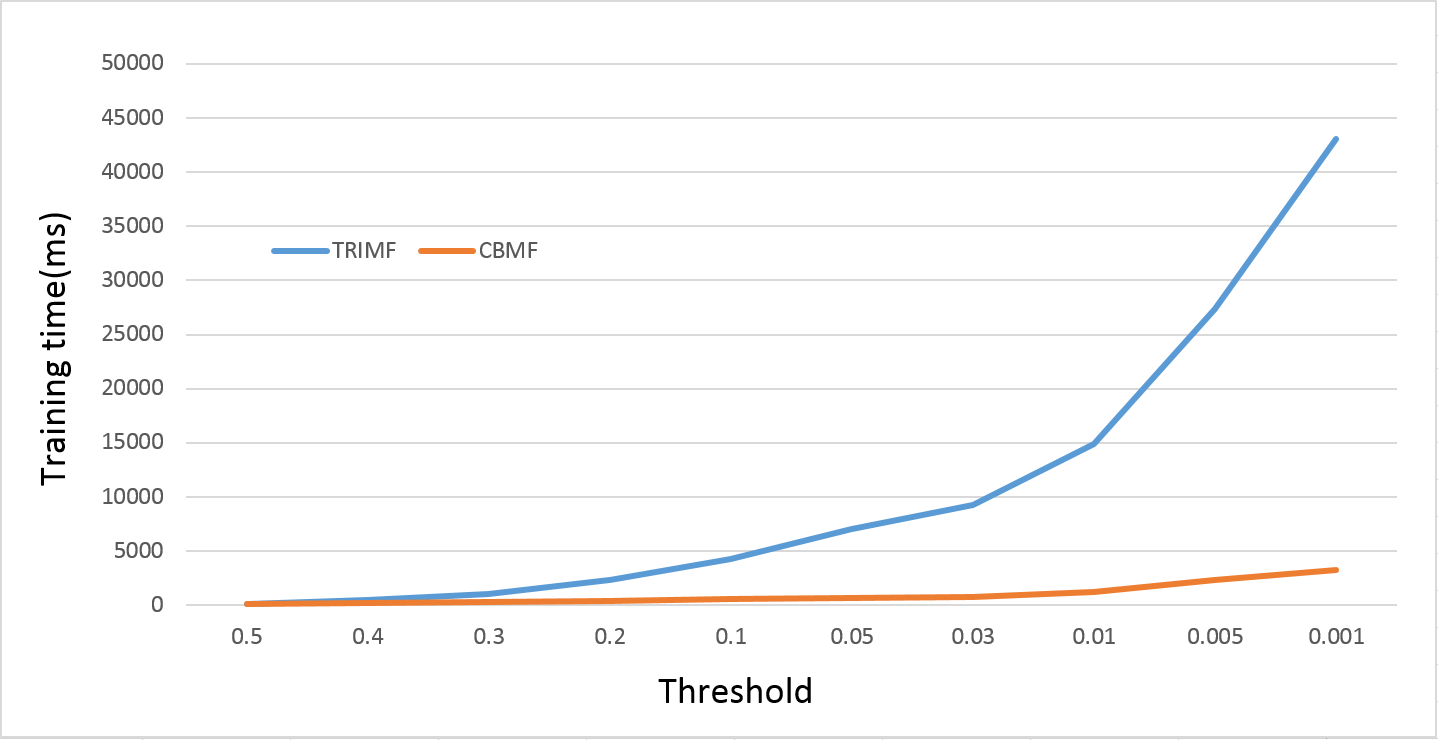
\includegraphics[width=0.9\textwidth]{fig/cbmf1.png} 
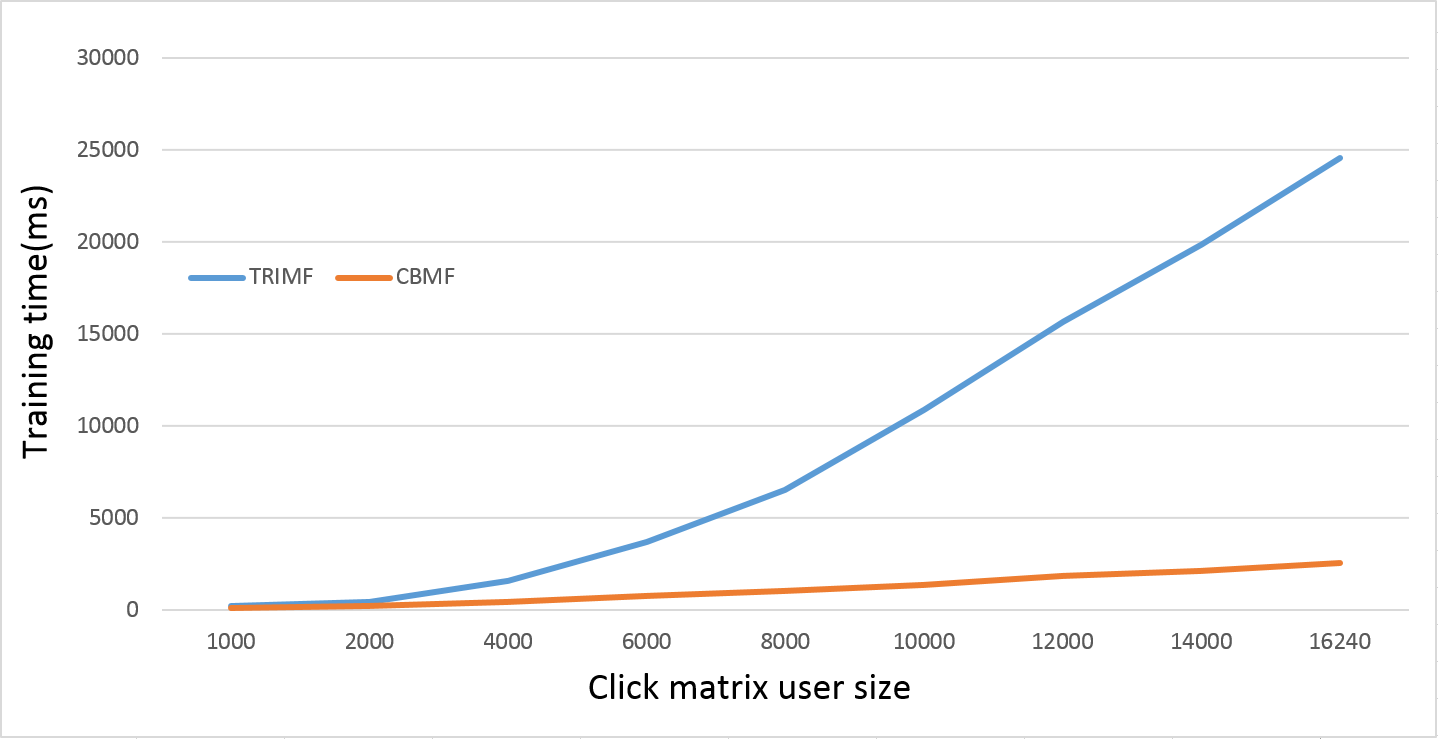
\includegraphics[width=0.9\textwidth]{fig/cbmf2.png} 
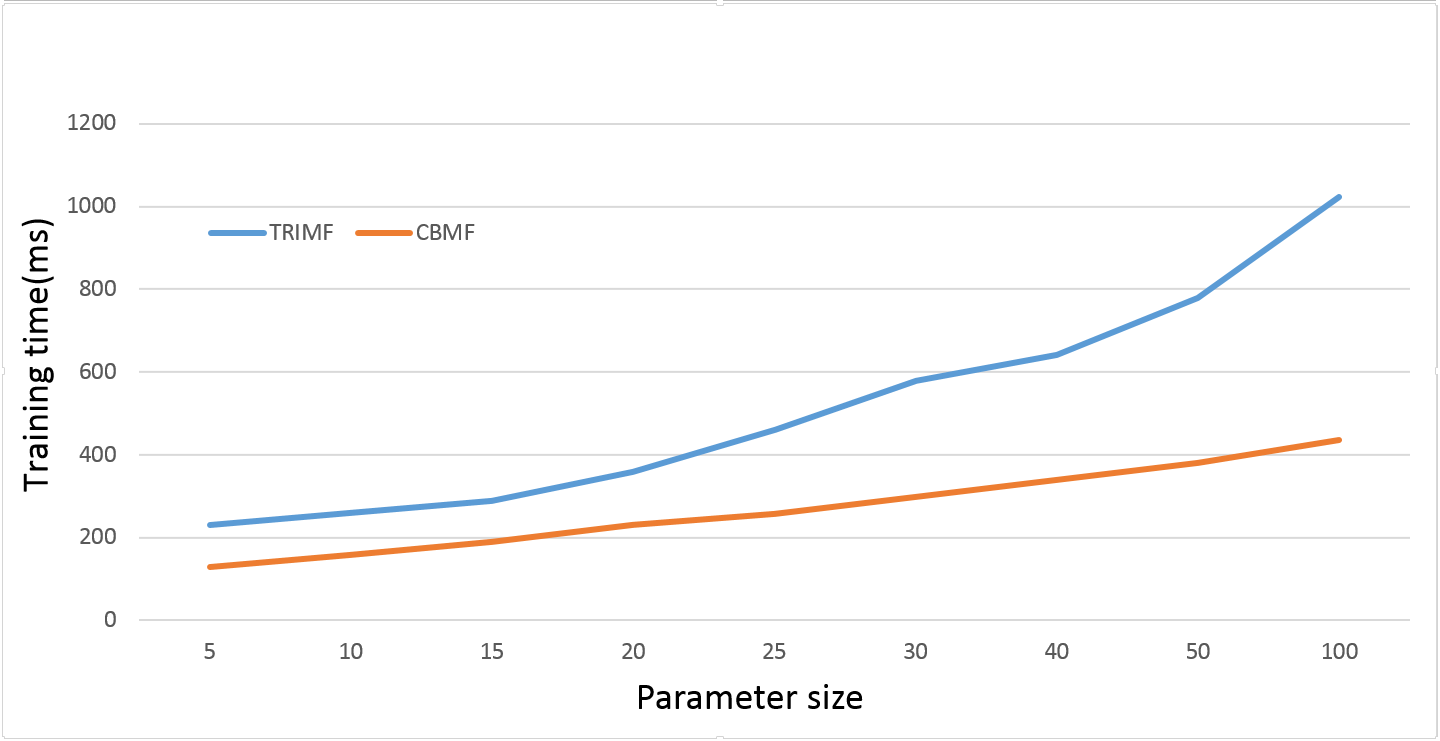
\includegraphics[width=0.9\textwidth]{fig/cbmfsize.png} 

\caption{scalability comparision between TRIMF and CBMF.}
\label{fig:cbmfall}
\end{center}
\end{figure}



In Figure \ref{fig:cbmfall}, we can see that CBMF runs significantly faster then TRIMF in every comparision. Which shows consistency with the time complexity of TRIMF and CBMF. In Table \ref{shortdeal} and \ref{longterm}, we see that the perfomance of CBMF and TRIMF are very close. Although TRIMF is slightly better in performance, but CBMF runs much faster and has good scalability. In online test, the data contains much more user and the latent dimension is larger. Therefore, we put CBMF online to perform tests.




\section{Online Experiments}


CBMF had been online for about one month from 2014-04-01 to 2014-05-01 with $20\%$ users, in the chatting scenario. That is, when you are chatting using QQ, an ad full of items will pop out in front of you. Most of the users will close it immediately, so $90\%$ of the users are new. We also need to provide results for every user;approximately 80,000,000.

After some days of parameter selection, CBMF's performance from 2014-04-10 stabilized. 

There are three evaluation metrics, all based on reactions to impressions. An impression is a measure of the number of times an advertisement is seen. 
\begin{itemize}
\item  click-through-rate(CTR). The click-through rate is the number of times a click is made on the advertisement divided by the total impressions (the number of times an advertisement was served). For example, if a banner ad is  delivered 100 times (100 impressions) and receives one click, then the click-through rate for the advertisement would be 1\%. $$CTR = \frac{Clicks}{Impressions} * 100\%$$
\item  order amount per impression(OAPI). The order amount per impression is the total price of orders divided by the total impressions. $$OAPI = \frac{Order \,\,Prices}{Impressions}$$
\item  pay amount per impression(PAPI). The pay amount per impression is the total price paid divided by the total impressions.$$PAPI = \frac{Paid \,\,Money}{Impressions}$$
\end{itemize}

These are three typical evaluation metrics in online test. CTR measures the success of an impression. While OAPI and PAPI directly reflect how much money is brought by recommendation. The difference between OAPI and PAPI is that a user may place an order but not pay (a cancellation can be made at any time).

\subsection{Baselines}

There are some others algorithms competing with CBMF, each covers $10\%-20\%$ percentage of the users. An ID is given to every algorithm, the ID of CBMF is 4312. The details of other algorithms are shown below:

\begin{itemize}

\item \textbf{Co-clustering CF} \cite{1565742}(4313) is a scalable collaborative filtering framework based on co-clustering. Previous work showed that this method had a fast training time while providing decent accuracy.
\item \textbf{Factorization Machine} \cite{/tist/LibFM-TIST12}(4314) is a generic approach that allows to mimic most factorization models by feature engineering. It provides high accuracy in several important prediction problems including recommender systems.
\item \textbf{Item-based CF} \cite{1167344}(4315) is a typical recommending method proposed by Amazon. Cosine distance is used in calculating item similarities.
\item \textbf{Efficient top-n recommendation} \cite{Aiolli:2013:ETR:2507157.2507189}(cpsf) is a recommendation pipeline, which is the winner of the Million Songs Dataset (MSD) challenge \footnote{http://www.kaggle.com/c/msdchallenge}
\item \textbf{CBMF}(4312): Our method.

\end{itemize} 

\subsection{Results}

\subsubsection{Click through rate}


\begin{figure}
\begin{center}
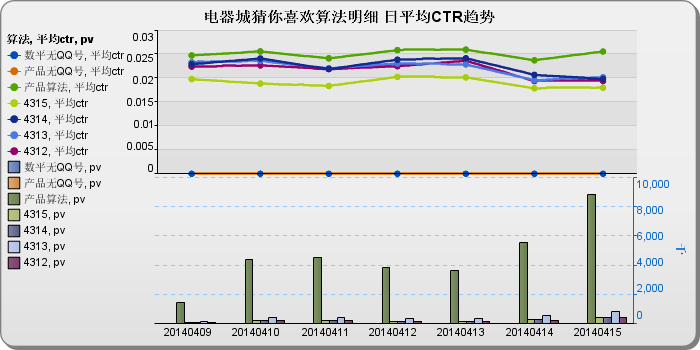
\includegraphics[width=400px]{fig/yixunexp/ctr0415.png}
\caption{\label{fig:ctr0415} CTR of online algorithms from 0409 to 0415.}

\end{center}
\end{figure}

\begin{figure}
\begin{center}

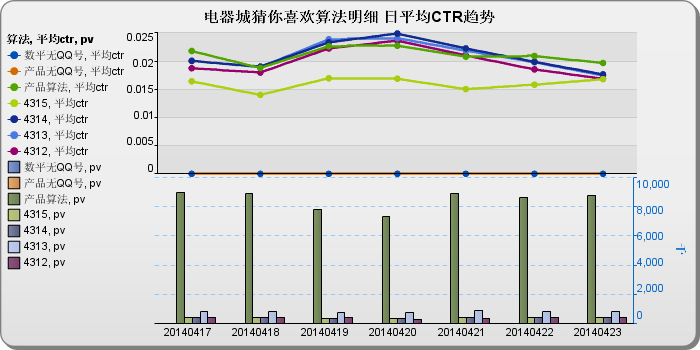
\includegraphics[width=400px]{fig/yixunexp/ctr0424.png}
\caption{\label{fig:ctr0424} CTR of online algorithms from 0417 to 0424.}
\end{center}
\end{figure}

In Figure \ref{fig:ctr0415} and Figure \ref{fig:ctr0424}, CTR of different online algorithms are shown. The id of CBMF is $4312$, the purple line. It can be seen that CBMF didn't rank first in CTR, but rather among the mid-levels. This is because CBMF didn't optimize for CTR, as it is designed for improving purchase rate. However, there is some similarity between click and purchase, so CBMF's CTR performance can be considered not too bad.

\subsubsection{Order amount per impression}

\begin{figure}
\begin{center}

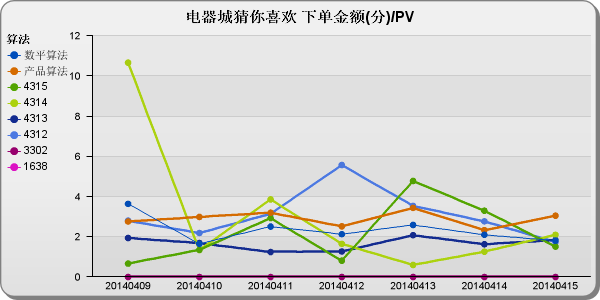
\includegraphics[width=400px]{fig/yixunexp/OAPI0415.png}
\caption{\label{fig:oapi0415} OAPI of online algorithms  from 0409 to 0415.}
\end{center}
\end{figure}

\begin{figure}
\begin{center}



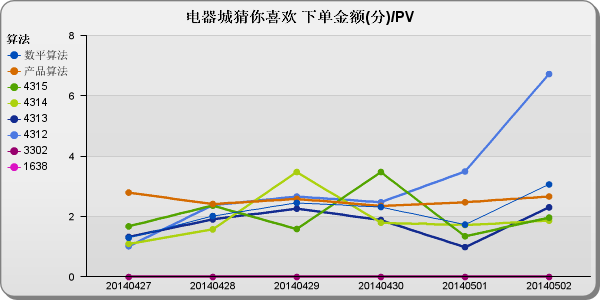
\includegraphics[width=400px]{fig/yixunexp/OAPI0427.png}
\caption{\label{fig:oapi0427} OAPI of online algorithms  from 0427 to 0502.}
\end{center}
\end{figure}

%\begin{figure}
%\begin{center}



%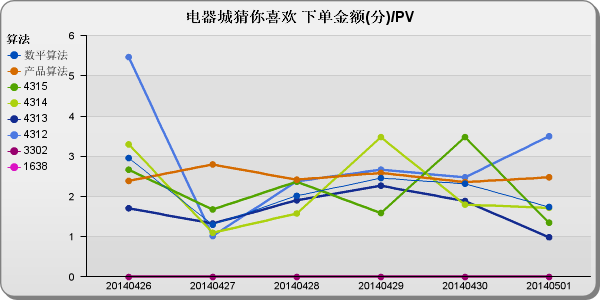
\includegraphics[width=400px]{fig/yixunexp/cvr0502.png}
%\caption{\label{fig:oapi0426} OAPI of online algorithms  from 0426 to 0501.}
%\end{center}
%\end{figure}

\begin{table}[h]

%\begin{Large}

\begin{center}
\begin{tabular}{| c | c | c | c |}
\hline
Algorithm ID & Average OAPI in Figure \ref{fig:ctr0415} & Average OAPI in Figure \ref{fig:ctr0424} & Average total OAPI \\
\hline
4315 &2.21 & 2.87 & 2.64\\
\hline
4314 &\textbf{3.33} & 2.65& 2.86\\
\hline
4312 &3.25& \textbf{3.97}& \textbf{3.65}\\
\hline
4313 & 1.93 & 2.31& 2.12\\
\hline
cpsf & 3.04& 2.98 & 3.01\\
\hline
\end{tabular}
\caption{\label{tbl:cvravg} Average OAPI of online algorithms.}
\end{center}
%\end{Large}
\end{table}

In Figure \ref{fig:oapi0415} and Figure \ref{fig:oapi0427}, OAPI of different online algorithms are shown. The id of CBMF is $4312$, the blue line. In Figure \ref{fig:oapi0415}, we can see that CBMF is relatively stable and its performance is among the best. In Figure \ref{fig:oapi0427} , CBMF outperforms other algorithms significantly. In Table \ref{tbl:cvravg}, we can see that although CBMF may not be the best in one week's performance due to insufficient data, its overall OAPI is the highest.

If we look at the figure carefully we can see that, CBMF tends to achieve better performance during holidays( 4-11, 4-12, 5-1, 5-2 are all Chinese holidays). This is because during holidays,  users tend to buy some things they have wanted for a long time. However, on ordinary days users may be inclined to buy only necessities. CBMF captures the users’ desire to buy something they like instead of what they need, so CBMF will achieve a better performance during holidays.

\subsubsection{Pay amount per impression}

\begin{figure}
\begin{center}

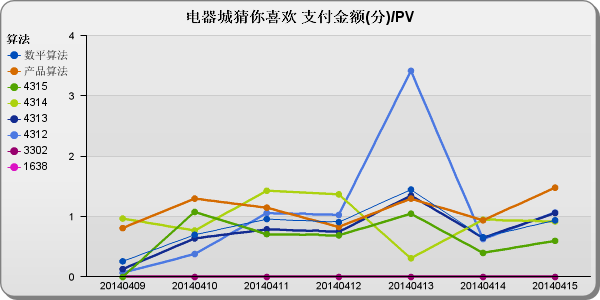
\includegraphics[width=400px]{fig/yixunexp/PAPI0415.png}
\caption{\label{fig:papi0415} PAPI of online algorithms  from 0409 to 0415.}
\end{center}
\end{figure}

\begin{figure}
\begin{center}

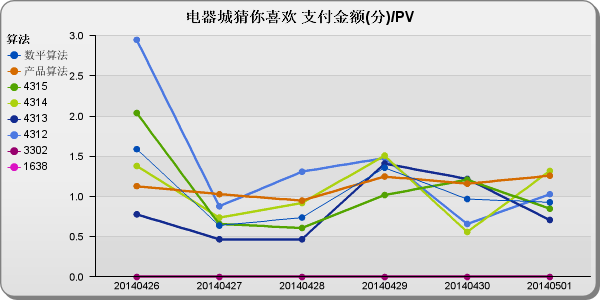
\includegraphics[width=400px]{fig/yixunexp/PAPI0421.png}
\caption{\label{fig:papi0501} PAPI of online algorithms  from 0426 to 0501.}
\end{center}
\end{figure}

In Figure \ref{fig:papi0415} and Figure \ref{fig:papi0501}, the OAPI of different online algorithms are demonstrated. The id of CBMF is $4312$, the blue line. We can see that CBMF outperforms other algorithms during these two periods. Different from the observations in OAPI, users may have a high OAPI on Mondays and Sundays, which might be because users may not have to pay right after they place their order. After thinking more carefully, they might eventually pay which would explain the delayed effect in the OAPI.

\subsection*{Overall Evaluation}
From the three evaluation metrics, we can see CBMF can achieve better conversion rates of the moderate click through rate compared to others.
